To define the network architecture of the solution to be created, some aspects must be remembered. One is that there are various communication technologies that may be used, as presented previously in Market Research. Other important aspect to keep in mind is that this solution implements both Smart Street Lighting and Smart Parking, through the use of street lampposts. So, these must have parking spots nearby, in order to allow full use of the Smart Parking feature. This lack of flexibility demands a creation of a network with nodes that may be far apart. Besides that, the data stream in the network will be very low since each lamppost will only communicate notifications on it's state. That is, if the lamp is light up, if it was detected a malfunction with the lamp, if it was detected an available parking space. 

With that in mind, through figure \ref{fig:LoRa_Range}, one can identify LoRa as a proper communication technology to use in this network.

\clearpage

\begin{figure}[ht]
	\centering
	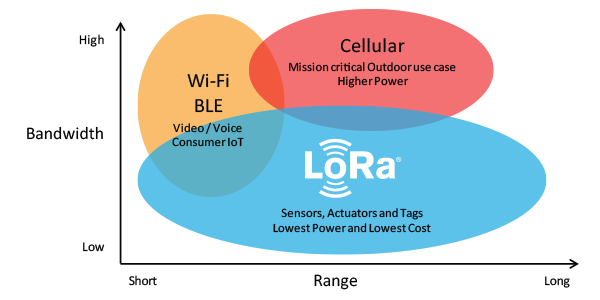
\includegraphics[width=0.70\textwidth]{/03system_overview/LoRa_Range}
	\caption{LoRa Range vs Bandwidth.}
	\label{fig:LoRa_Range}
\end{figure}

In figure \ref{fig:network_arch} one can see the network architecture diagram. This is a star topology, in which the gateway relay messages between each local system (lamppost) and a central network server, the remote system. This wireless communication takes advantage of the Long Range characteristics of the LoRa physical layer, allowing a single-hop link between the local system and the gateway. All communication modes are capable of bi-directional communication, and there is support for multicast addressing groups. The gateway is connected to the internet in order to store new information about the network in a remote system.

\begin{figure}[ht]
	\centering
	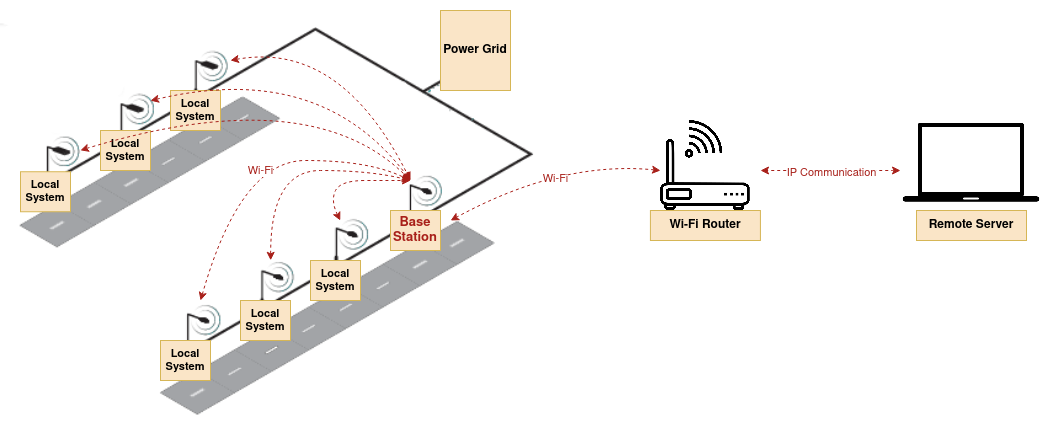
\includegraphics[width=1\textwidth]{/03system_overview/network_arch}
	\caption{Network architecture.}
	\label{fig:network_arch}
\end{figure}
\clearpage


%That being said, if each lamppost is spaced by 4 meters, each base station can easily connect with 10 local systems. To communicate with a remote server, the gate will be connected to the internet through an Ethernet cable, or similar, that will most certainly already exist near the lampposts, in the telecommunications infrastructure.

